\documentclass[letterpaper,12pt]{extarticle}
\usepackage{astro-mini}
\usepackage{lipsum}


\usepackage{array}   % for \newcolumntype macro
% math-mode version of column types
\newcolumntype{L}{>{$}l<{$}}
\newcolumntype{C}{>{$}c<{$}}
\newcolumntype{R}{>{$}r<{$}}


\begin{document}

\begin{center}

    \Large Estudio de variables irregulares: Mira y T. Tauri
    
    \vspace{3mm}

    \large Juan David Aparicio Gutiérrez

    \vspace{3mm}
    \normalsize 
\end{center}


\section{Introducción}

Las estrellas variables constituyen un laboratorio natural para el estudio de procesos físicos estelares a diferentes escalas evolutivas. En particular, el análisis de sus curvas de luz permite caracterizar mecanismos de pulsación, rotación, acreción y estructuras circumestelares mediante la identificación de periodicidades dominantes y modulaciones de largo plazo. En este contexto, la determinación del período envolvente de una señal fotométrica resulta especialmente útil cuando la variabilidad no es estrictamente periódica, sino que presenta cambios de amplitud o modulaciones temporales superpuestas a la señal principal.

Entre las variables pulsantes de gran amplitud se encuentran las estrellas tipo Mira, que corresponden a gigantes rojas muy frías, con temperaturas cercanas a los $3000,\mathrm{K}$, radios del orden de cientos de radios solares y luminosidades que pueden alcanzar miles de veces la del Sol. Como describe \cite{mattei1997}, estas estrellas presentan períodos largos, típicamente entre 150 y 1000 días, y amplitudes fotométricas superiores a $2.5$ magnitudes en el visible, asociadas a pulsaciones radiales en etapas avanzadas de la evolución estelar. Sin embargo, sus curvas de luz no son estrictamente periódicas: tanto el período como la amplitud pueden variar de ciclo a ciclo, lo que hace necesario el uso de herramientas que permitan caracterizar modulaciones lentas o tendencias envolventes en la señal observada.

Por otra parte, las estrellas T Tauri representan objetos jóvenes de pre–secuencia principal con masas menores a aproximadamente $2,M_\odot$, cuya variabilidad fotométrica está dominada por múltiples procesos físicos simultáneos. Como explican \cite{elizabethson2023}, entre estos mecanismos se encuentran la acreción desde discos protoplanetarios, la presencia de manchas frías y calientes en la superficie estelar, la rotación diferencial, la interacción con material circumestelar y eventos eruptivos asociados a reconexión magnética. Estos fenómenos producen curvas de luz con morfologías complejas y escalas temporales diversas, que pueden incluir componentes periódicas, cuasiperiódicas y estocásticas, dificultando la identificación de un período característico único.

Debido a esta complejidad, el análisis de curvas de luz de estrellas tipo Mira y T Tauri requiere técnicas que permitan identificar no solo periodicidades dominantes, sino también variaciones de amplitud en escalas temporales mayores. En este laboratorio se estudiarán estas modulaciones mediante la estimación del período envolvente de las señales fotométricas, con el objetivo de caracterizar la estructura temporal de la variabilidad y comparar su comportamiento en estrellas evolucionadas pulsantes y en objetos jóvenes de pre–secuencia principal.

\section{Objetivos}

\begin{itemize}
    \item Identificar la periodicidad de pulsación dominante en curvas de luz de estrellas tipo Mira mediante el periodograma de Lomb-Scargle.
    \item Detectar y caracterizar modulaciones de largo plazo en las curvas de luz de estrellas Mira mediante el ajuste de un modelo de serie de Fourier y la posterior sustracción de la tendencia envolvente.
    \item Evaluar el efecto del proceso de \textit{detrending} sobre la curva de luz doblada en fase, comparando la dispersión de la señal antes y después de remover la componente de largo período.
    \item Estimar el período envolvente de la estrella T~Tauri TIC~264739351 a partir de datos fotométricos de TESS, utilizando el análisis de Lomb-Scargle y la comparación visual de curvas dobladas en fase.
    \item Comparar la naturaleza de la variabilidad periódica en estrellas evolucionadas (tipo Mira) y objetos jóvenes de pre-secuencia principal (T~Tauri), relacionando los resultados con los mecanismos físicos subyacentes en cada clase estelar.
\end{itemize}

\section{Procedimiento}

\subsection{Estrellas tipo Mira}

Se seleccionaron los cinco archivos de mayor tamaño del directorio de datos, correspondientes a las curvas de luz con mayor número de observaciones. Las magnitudes fueron centradas restando su valor medio antes de cualquier análisis espectral.

La identificación de la periodicidad corta dominante se realizó mediante el periodograma de Lomb-Scargle (método \textit{fast}) aplicado al rango de frecuencias determinado automáticamente. La frecuencia con mayor potencia espectral se tomó como la frecuencia de pulsación principal, $f_{\rm corta}$.

Para caracterizar la modulación de largo plazo, se restringió el barrido de frecuencias al intervalo $[1/T_{\rm span},\, f_{\rm corta}/\mathrm{lpf}]$, donde $T_{\rm span}$ es la duración total de la serie y $\mathrm{lpf}$ (\textit{long period factor}) es un parámetro que garantiza la separación entre ambas componentes. El pico de mayor potencia en este subrango se identificó como la frecuencia de la envolvente larga, $f_{\rm larga}$.

Con $f_{\rm larga}$ se ajustó una serie de Fourier truncada a $N_{\rm terms} = 2$ términos, obteniendo un modelo analítico de la tendencia de largo plazo. Este modelo se restó a la curva original (\textit{detrending}). La curva de luz se presentó doblada en fase tanto con como sin detrending, junto con la serie temporal y el modelo de tendencia superpuesto.

\subsection{Estrella T Tauri}

Para la estrella T Tauri TIC~264739351, observada por TESS, se construyó una grilla de frecuencias uniforme desde $1/T_{\rm span}$ hasta $1/0.1\,\mathrm{d}^{-1}$, con una resolución de $30\times T_{\rm span}$ puntos. El periodograma de Lomb-Scargle se calculó con el método \textit{fastchi2} y se normalizó respecto a su valor máximo. Los picos del periodograma fueron identificados con \texttt{scipy.signal.find\_peaks}, y se seleccionaron los diez de mayor potencia como candidatos a frecuencias significativas.

Dado que la variabilidad de las T Tauri puede estar dominada por una modulación de largo plazo, se extrajeron los tres picos de menor frecuencia (mayor período) entre todos los detectados. Para cada candidato se generó su curva de luz doblada en fase y el periodograma del residuo tras sustraer el modelo sinusoidal correspondiente a esa frecuencia. La comparación visual de las curvas dobladas y de los residuos permitió seleccionar la frecuencia envolvente más representativa.

\section{Problemas presentados y soluciones aplicadas}

\subsection{Estrellas tipo Mira}

El principal desafío en el análisis de las estrellas Mira fue la calibración del modelo de Fourier empleado para representar la tendencia de largo plazo. Dado que una serie con muchos términos puede sobreajustar la señal e incorporar parte de la variabilidad de corto plazo, fue necesario determinar empíricamente el número óptimo de términos. Tras evaluar distintas configuraciones, se encontró que $N_{\rm terms} = 2$ ofrecía el mejor balance entre fidelidad a la envolvente y suavidad del modelo, sin capturar oscilaciones propias de la pulsación principal.

Un segundo problema estuvo asociado al parámetro $\mathrm{lpf}$. Este factor define el límite superior de frecuencias en la búsqueda del período largo, exigiendo que $T_{\rm largo} > \mathrm{lpf}\times T_{\rm corta}$; sin embargo, la cota superior está acotada por el rango temporal disponible: si $\mathrm{lpf}$ es demasiado grande, el rango de búsqueda queda vacío y no es posible detectar una modulación larga. Dado que no era posible extender las observaciones, se priorizó obtener el mejor resultado dentro de las restricciones impuestas por la duración de cada serie de tiempo y la complejidad propia de la curva de luz.

\subsection{Estrella T Tauri}

En el caso de la estrella T Tauri, la dificultad principal residió en la escasez de picos prominentes en el periodograma para períodos largos. Inicialmente, el barrido de frecuencias no se extendía lo suficiente hacia las frecuencias bajas, lo que limitaba la detección de variabilidades de largo período. Para resolver esto, se amplió el rango de períodos de prueba hasta el máximo posible, es decir, hasta la duración total de la serie ($T_{\rm span}$). Aún con esta extensión, la identificación de una frecuencia envolvente única resultó ambigua. Partiendo del supuesto de que la modulación dominante corresponde a una frecuencia muy baja, se optó por seleccionar los tres picos de menor frecuencia detectados, sustraer el modelo sinusoidal asociado a cada uno y comparar visualmente tanto las curvas dobladas en fase como los periodogramas residuales, eligiendo finalmente la configuración que producía una curva más coherente y un residuo con menor estructura remanente.

\section{Resultados}

Se analizaron las variables Mira con identificador OGLE-BLG-LPV 003971, 005545, 005621, 124320 y
176699. La serie de tiempo completa y las dos curvas faseadas para cada una se muestran
en las figuras \ref{fig:mira1}, \ref{fig:mira2}, \ref{fig:mira3}, \ref{fig:mira4} y \ref{fig:mira5}, junto con los dos períodos obtenidos.

\begin{figure}[H]
	\centering
	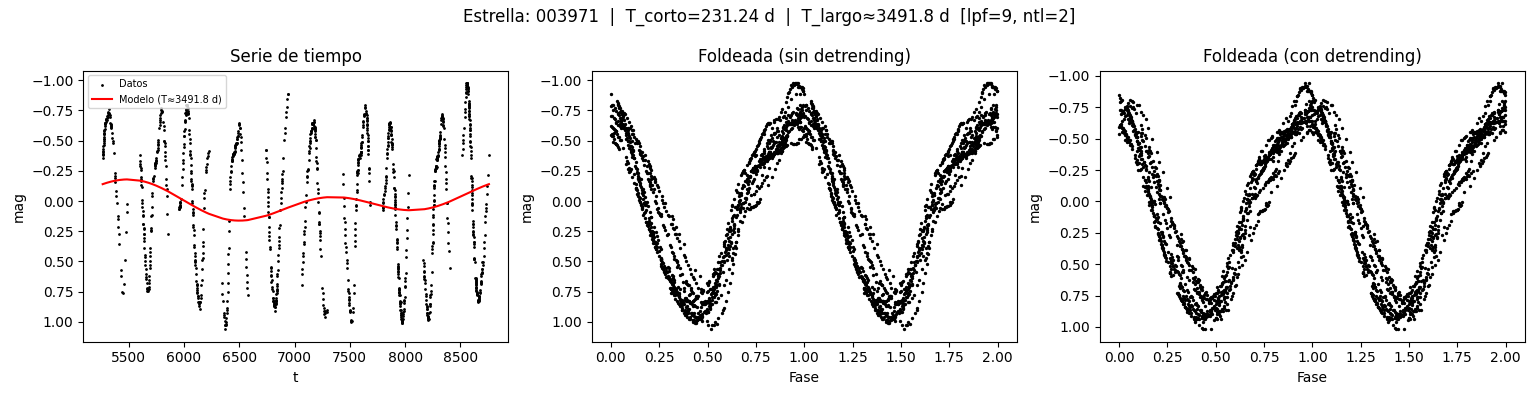
\includegraphics[width=\textwidth]{img/mira_003971.png}
	\caption[Mira 003971]{
		Serie de tiempo, curva de luz foldeada original, y 
        curva de luz foldeada con la frecuencia envolvente restada.
	}
	\label{fig:mira1}
\end{figure}

\begin{figure}[H]
	\centering
	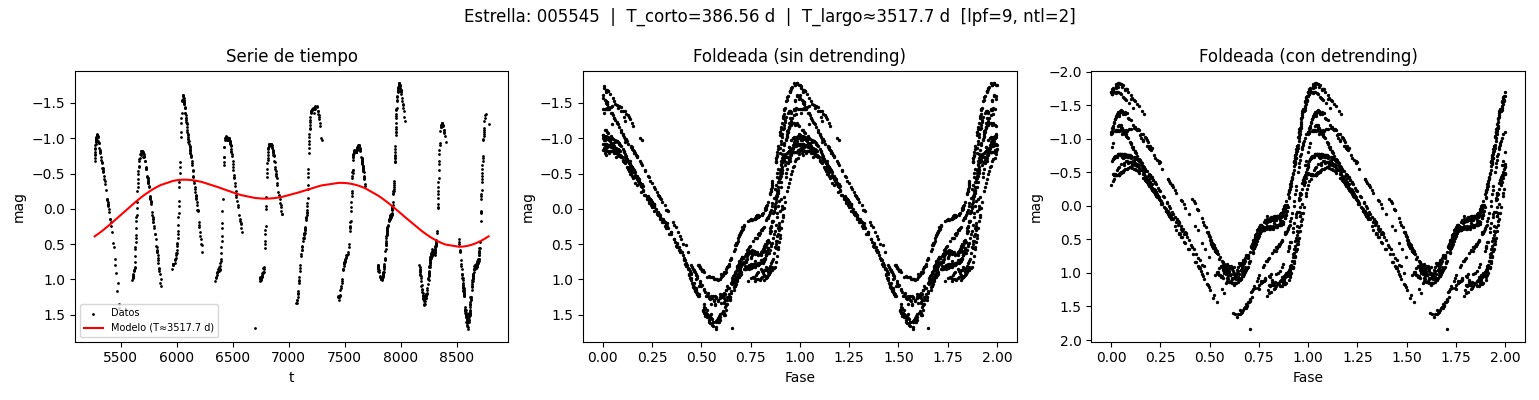
\includegraphics[width=\textwidth]{img/mira_005545.png}
	\caption[Mira 005545]{
		Serie de tiempo, curva de luz foldeada original, y 
        curva de luz foldeada con la frecuencia envolvente restada.
	}
	\label{fig:mira2}
\end{figure}

\begin{figure}[H]
	\centering
	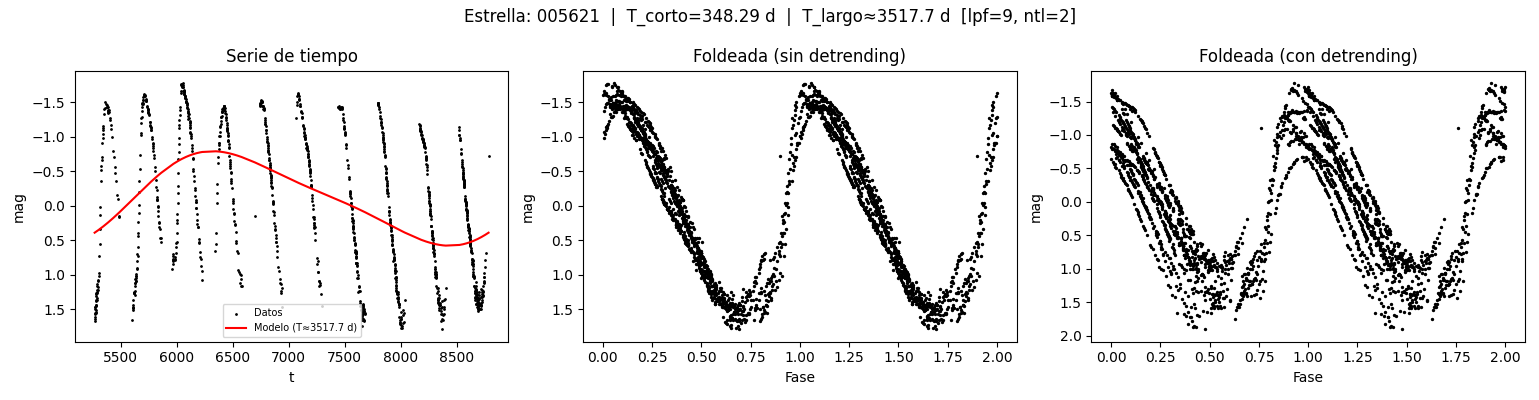
\includegraphics[width=\textwidth]{img/mira_005621.png}
	\caption[Mira 005621]{
		Serie de tiempo, curva de luz foldeada original, y 
        curva de luz foldeada con la frecuencia envolvente restada.
	}
	\label{fig:mira3}
\end{figure}

\begin{figure}[H]
	\centering
	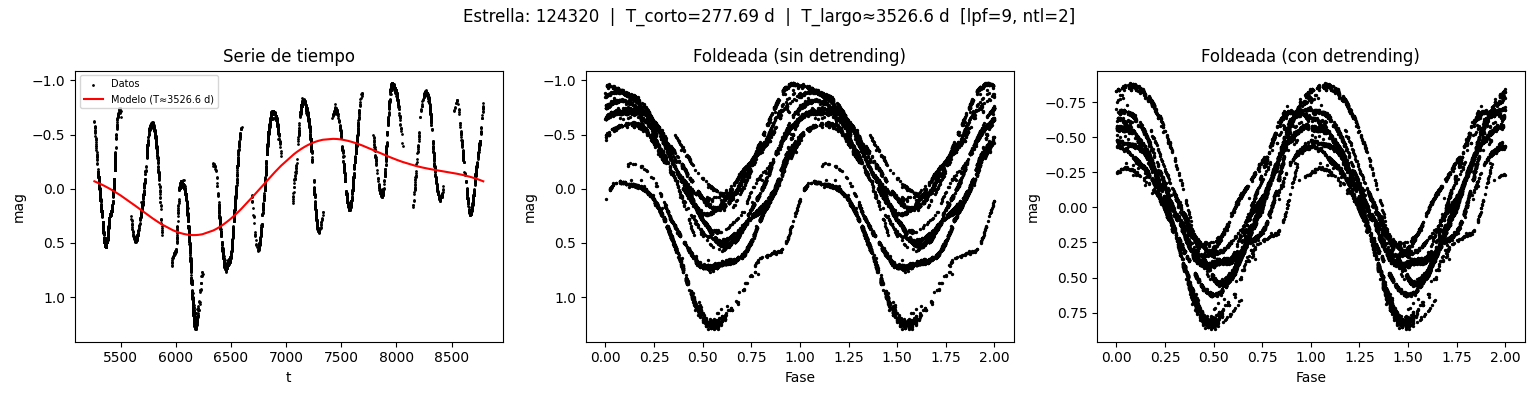
\includegraphics[width=\textwidth]{img/mira_124320.png}
	\caption[Mira 124320]{
		Serie de tiempo, curva de luz foldeada original, y
        curva de luz foldeada con la frecuencia envolvente restada.
	}
	\label{fig:mira4}
\end{figure}

\begin{figure}[H]
	\centering
	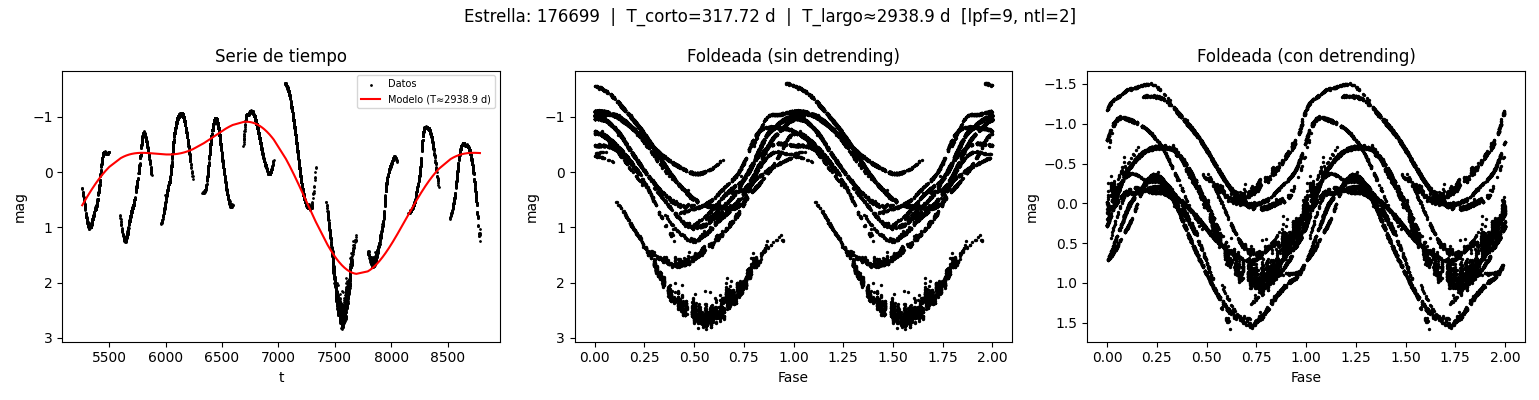
\includegraphics[width=\textwidth]{img/mira_176699.png}
	\caption[Mira 176699]{
		Serie de tiempo, curva de luz foldeada original, y
        curva de luz foldeada con la frecuencia envolvente restada.
	}
	\label{fig:mira5}
\end{figure}

La serie temporal de la T. Tauri se muestra en la figura \ref{fig:ttauri_timeseries}.
El período corto encontrado fue de 2.18 días, mientras que el período
de modulación larga fue de 10.89 días.
El período largo fue seleccionado entre los candidatos mediante
comparación visual de las curvas dobladas en fase, eligiendo
aquel cuya curva presentaba mayor coherencia morfológica.
La curva de luz foldeada en el período corto junto con el periodograma
de Lomb-Scargle se muestran en la figura \ref{fig:ttauri}. Se probaron
tres frecuencias como candidatas a envolvente, y los resultados
de cada prueba se presentan en las figuras \ref{fig:test1},
\ref{fig:test2} y \ref{fig:test3}.

\begin{figure}[H]
	\centering
	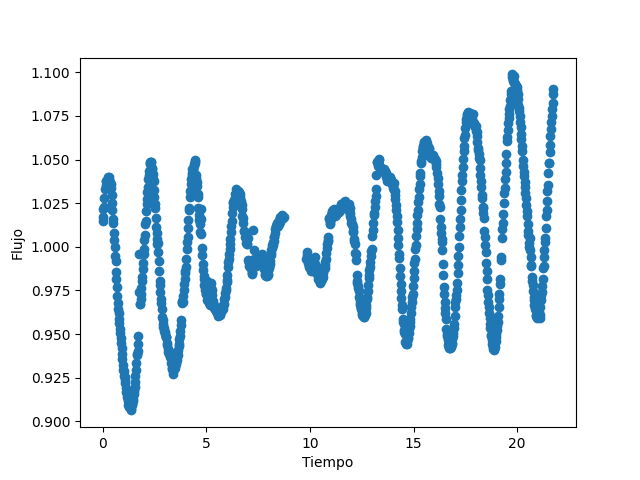
\includegraphics[width=\textwidth]{img/ttauri_timeseries.png}
	\caption[Serie de tiempo de la T. Tauri]{
		Serie de tiempo de la T. Tauri TIC 264739351.
	}
	\label{fig:ttauri_timeseries}
\end{figure}

\begin{figure}[H]
	\centering
	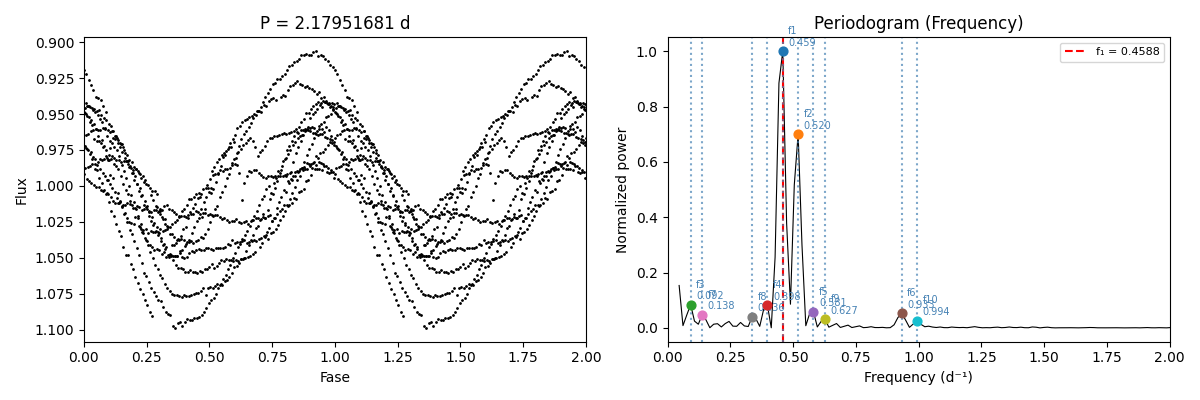
\includegraphics[width=\textwidth]{img/ttauri.png}
	\caption[Folding T. Tauri]{
		Curva foldeada en el período corto de la T.Tauri.
	}
	\label{fig:ttauri}
\end{figure}

\begin{figure}[H]
	\centering
	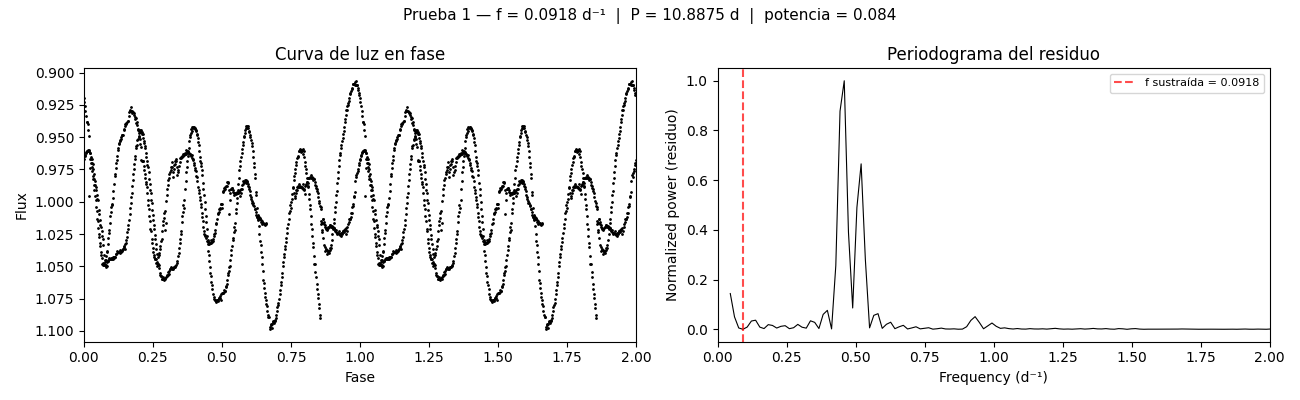
\includegraphics[width=\textwidth]{img/ttauri_test1.png}
	\caption[Test 1]{
		Curva de luz foldeada y nuevo
        periodograma de Lomb-Scargle para la
        primera frecuencia candidata a envolvente.
	}
	\label{fig:test1}
\end{figure}

\begin{figure}[H]
	\centering
	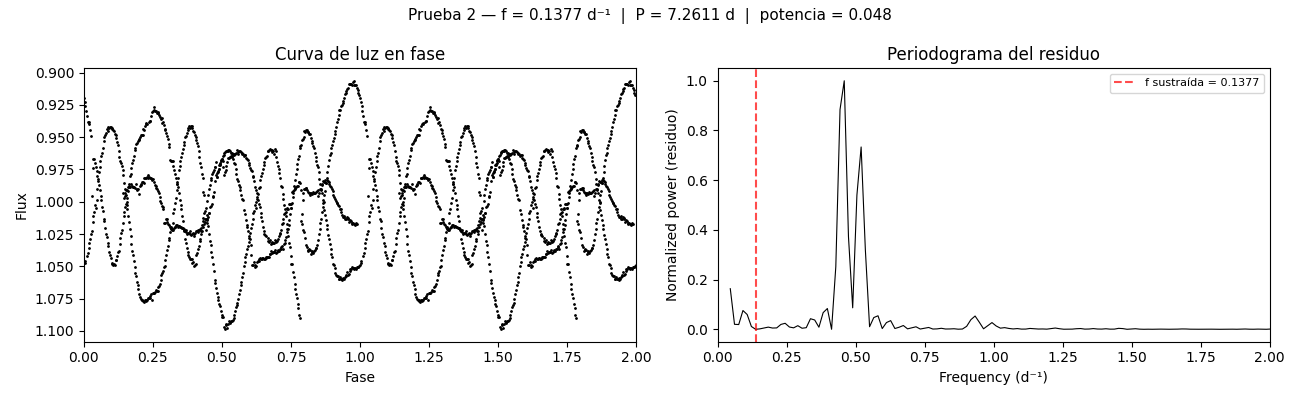
\includegraphics[width=\textwidth]{img/ttauri_test2.png}
	\caption[Test 2]{
		Curva de luz foldeada y nuevo
        periodograma de Lomb-Scargle para la
        segunda frecuencia candidata a envolvente.
	}
	\label{fig:test2}
\end{figure}

\begin{figure}[H]
	\centering
	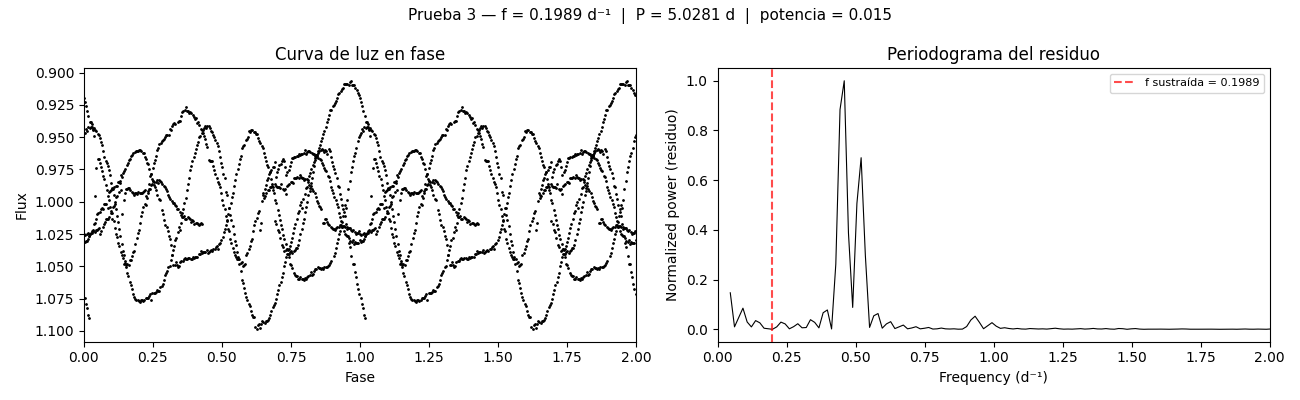
\includegraphics[width=\textwidth]{img/ttauri_test3.png}
	\caption[Test 3]{
		Curva de luz foldeada y nuevo
        periodograma de Lomb-Scargle para la
        tercera frecuencia candidata a envolvente.
	}
	\label{fig:test3}
\end{figure}

\section{Conclusiones}

El análisis de las cinco estrellas tipo Mira del catálogo OGLE permitió identificar, en todos los casos, dos componentes periódicas bien diferenciadas: una pulsación dominante de corto período, característica de estas gigantes rojas en etapas avanzadas de la evolución estelar, y una modulación de largo plazo asociada a variaciones lentas en la amplitud y la forma de la curva de luz. La sustracción del modelo de Fourier de dos términos resultó suficiente para capturar la tendencia envolvente sin absorber la variabilidad de corto período, y las curvas dobladas en fase mostraron una mejora visible en coherencia tras el proceso de \textit{detrending}. Esto confirma la naturaleza biperiódica de estas variables y la utilidad del enfoque combinado Lomb-Scargle más ajuste armónico para separar ambas componentes.

En el caso de la estrella T~Tauri TIC~264739351, se identificó un período corto de $2.18$ días, consistente con la escala temporal de rotación estelar, y un período de modulación larga de $10.89$ días, seleccionado a partir de la comparación visual de tres candidatos de baja frecuencia. A diferencia de las Mira, la variabilidad de esta estrella joven resultó más irregular y con menor amplitud relativa entre componentes, lo que refleja la superposición de múltiples mecanismos físicos —rotación, acreción, manchas estelares— tal como se describe en la literatura para objetos de pre-secuencia principal.

En términos comparativos, ambas clases estelares presentan variabilidad con estructura multiescala temporal, pero con orígenes físicos y grados de regularidad notablemente distintos. Mientras que las Mira exhiben pulsaciones radiales cuasiperiódicas con modulaciones de amplitud bien definidas, la curva de luz de la T~Tauri refleja una dinámica más estocástica que dificulta la identificación unívoca de un período envolvente. El presente laboratorio evidencia cómo la elección de la metodología de análisis debe adaptarse a la naturaleza de cada objeto: el detrending por series de Fourier es adecuado para las Mira, en tanto que para las T~Tauri el análisis iterativo de residuos del periodograma junto con la comparación visual resulta más apropiado ante la ausencia de una modulación larga bien definida.

% Bibliography
\footnotesize

\bibliographystyle{aa_url} % style aa.bst
\bibliography{global.bib}




\end{document}




